
%(BEGIN_QUESTION)
% Copyright 2013, Tony R. Kuphaldt, released under the Creative Commons Attribution License (v 1.0)
% This means you may do almost anything with this work of mine, so long as you give me proper credit

Sketch connecting wires to allow this data acquisition (DAQ) module to indicate light intensity at input channel {\tt IN 1} (i.e. more light results in a stronger positive reading at the DAQ).  Feel free to add any additional components you deem necessary to this circuit!

\vskip 50pt

$$\includegraphics[width=15.5cm]{i03470x01.eps}$$

\underbar{file i03470}
%(END_QUESTION)





%(BEGIN_ANSWER)

Any solution where DAQ input channel \#1 senses an increasingly positive voltage as photocell resistance decreases (photocell is illuminated) is correct:

$$\includegraphics[width=15.5cm]{i03470x02.eps}$$

%(END_ANSWER)





%(BEGIN_NOTES)

{\bf This question is intended for exams only and not worksheets!}.

%(END_NOTES)

